\documentclass{article}
\usepackage[utf8]{inputenc}
\usepackage[letterpaper, margin=2in]{geometry}
\usepackage{amsmath}
\usepackage{upgreek}
\usepackage{sectsty}
\usepackage{lmodern}
\usepackage{todonotes}
\usepackage{graphicx}
\graphicspath{ {images/} }
\allsectionsfont{\centering}
\linespread{1.05}
\title{Cell Phones Final Paper}
\author{Bosco Ndemeye\\ Jonathan Kwee}
\date{November 2016}

\begin{document}

\maketitle

\section{Introduction}
From the invention of the portable cell phone in 1973, cell phones remained very expensive till the end of the 1980s. During the 1990s however, the technological advances of the time allowed cell phone designers to develop more compact designs which made the cell phones easy to carry and much cheaper. Consequently, as time progressed this allowed huge portions of the population to gain easy ownership of the phones. \par It goes without saying, that cell phones have had a big positive impact on our world. From their help to connecting our world in ways one could not have imagined before, to helping us save lesser and lesser amounts of money through phone-applications. With so much positive influence on the world around us however, what we often fail to ask ourselves is how much negative change this cell phone revolution might have brought to this world. In this paper we will explore one possible negative aspect of the cell phone revolution. Using two different models of computation, we investigate the ways in which the cell phone revolution has contributed to the changes in energy consumption over the years.  We will take the approach described below. \par 
Taking USA as our model, assume that all members of a past land-line owning family now have a cell phone. We will call the period of time when not all the members possess cell-phones the \textit{transition state}, whereas the period of time when they all do will be referred to as \textit{steady state}. Then, we calculate the amount of energy that was spent due to cell phones from the starting state through the transition state up until the steady state. Among other things, as one would guess, we observe that there has been an overall increase in energy consumption due to cell phone service since the cell phone was invented. Moreover, and probably more interestingly, we find that if the increase in energy consumption was due to population growth alone, the energy increase would be almost linear. However, by considering how owner-ship of cell phones have changed  throughout the years, by including the \textit{popularity index}\footnote{The higher this is, the more people tend to buy cell-phones. It was calculated based on data  about the amount of people per year, that had cell phone plans from 1985 to 2010 \cite{subscribers}} in our model,
the graph becomes exponential, by using one model and slightly logarithmic by using another model. The models and their differences are discussed in a later section.
. 

\section{Background}
A number of articles and publications have been dedicated to the cell phone revolution. However, most researches into this area focus more on social issues associated with the cell phone revolution. For example: there is a lot of research about smart-phone and cell phone usage in different races, different regions of the globe etc. These, even though they are important, discuss an issue that is very different from what we want to investigate, and are therefore irrelavant . One paper that seems to be concerned with the same energy issue like we are is \textit{The investigation on the Revolution and Need of Energy Efficient Smart-phone Development} \cite{phoneBatteries}. The authors discuss how cell phone batteries have evolved over the years and why this was so. However, they do not, like us, present any interest in investigating the impact of this cell phone battery evolution on the amount of energy that is being consumed today. Our paper aims to provide a strong case about how the increase in the amount of energy used over the recent years has been partly due to the increase in the power and amount of digital devices, specifically cell phones. 


\section{Model Descriptions}
This paper considers and compares two models of computation where from each model important conclusions about population growth, and energy used or wasted over the years are drawn. Specifically we will use \textbf{\textit{Differential Equations Modeling}}  and \textbf{\textit{Monte Carlo Simulation}}. \par
Conceptually, \textit{Differential Equations Modeling} looks at a problem in terms of whole populations' rates of change, comes up with differential equations describing his/her system, and using numerical methods of integration, solves the differential equations. From the results, he/she can choose to visualize the data in terms of graphs or just present his numerical results as they  are. In our case, we will visualize and analyze our results based on the graphs we will have produced.\par 
On the other hand, \textit{Monte Carlo Simulation} simulates a situation with a range of estimates. One random value chosen from the range is inputted into the simulation as a run. The results are based upon numerous runs using multiple random values. Unlike the Differential Equations Modeling whose main components are the differential equations, Monte Carlo Simulation's key feature is the range of estimated values. These range of values will directly affect the risk and uncertainty of the model. However, if the range of estimates are well calculated, then the model will show us the likeliness of the result happening in the future.\par
Briefly, our approach using Monte Carlo Simulation starts with a simulation of one household. This model will take a list of parameters: \textit{Amount of Cellphones in the Household}, \textit{Amount of Landlines in the Household}, \textit{Battery Capacity of Cellphones}, \textit{Energy Consumption of Landlines} and a variable called \textit{Popularity Index}. Using these variables, our model will show the total amount of energy consumed in a day. Each household is also given a random number which will be used in relation to the popularity index to determine whether that particular household would obtain a cellphone. To simulate the whole United States, we expand on this household to the amount of household in the US in any given point of time. We also decided to limit our calculations for energy consumption to a per day basis instead of a per year basis since both ways will show the same conclusion but at a different scale.\par
Similarly, our differential equations model the changes in four types of populations over time, \textit{The total number of landline-owning households in the US, the total number of cell-phone-owning households in the US, the total number of households, as well as the total number of households which are still transitioning from owning landlines to owning cell-phones}. The specifics of this are described in detail in Section 3.2. \par
%Now that we have a conceptual understanding of  the two models we are going to consider, and the conceptual differences between them, in the next few sub-sections, we will describe how each model has been used in the solution to our cell phone revolution energy problem. 

\subsection{Monte Carlo Simulation}
In the starting state, Let the number of land-line owning households in the USA be $H$. Let  there be 3  members  within each household. \footnote{based on the average size of household in the US. \cite{Households}}    \par
We know that in the starting state, there are no cell phones, so the number, $c$, of cell phones in a household is zero, whereas we assume that each household contains exactly one landline. Therefore if $l$ signifies the amount of landlines, then in the starting state, $l = H$. We let the total amount of energy consumed by one landline per hour be 2.5 (W/h) \cite{chargerData} so throughout the course of a day, the total energy consumed per landline is $2.5 \cdot 24~ W$. Let this constant be $e_l$, then, we have the following equation:
$$ \text{\textbf{Total energy consumed in the starting state: }} E = (l \cdot e_l) \cdot H \cdot D$$ where $D$ is the number of Days.\\

Figuring out the amount of energy that was spent in the United States before the invention of the cell phone was the easy part. The difficult part is finding how much  the invention of the cell phone added to the amount of energy that was consumed everyday throughout the United States over the years. To do this, we are going to take a step by step approach to the solution of our problem.

\subsubsection{Assume The Cell Phone Was Never Invented}
If we are going to learn about how much change the cell phone revolution added to the amount of energy we could have been consuming, it only seems reasonable to have a figure to compare to. \par 
If the cell-phone was never invented, the increase in energy consumed today would have solely been due to the increase in population. Thus, calculating the amount of energy that phone service was consuming would just be a matter of taking the average amount of energy consumed by one landline per day and multiplying it by the number of landlines in the whole US at a specific time period. Using data from Statista \cite{Households} we did this and found the total energy consumed due to landlines in a day throughout the years, described on Figure \ref{1}.
\\
\begin{figure}
  \makebox[\textwidth][c]{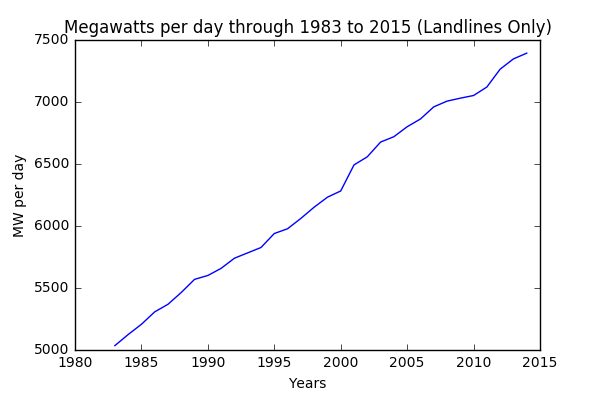
\includegraphics[width=\textwidth]{LandlineOnly.png}}%
  \caption{Energy Consumed due to Population Growth}
  \label{1}
\end{figure}


As we can see from the graph, if the cell phone was never invented, in 2015 the amount of energy due to using phone service would have been $7500 \text{MW}$. Moreover, note how the rate of change of energy throughout the years is linear! \par
Using regression analysis from Python's Scipy module, this graph has an r-value of $0.9977$ which suggests a near perfect positive linear relationship, a slope of $76.6$ and a y-intercept of -146854. In layman terms, throughout the years, there is no doubt that the population growth increases the energy spending of the US. Using the slope and the y-intercept, we form an equation that can predict the amount of energy spent in the later years if the population growth is consistent.
$$ E(t) = 76.6t - 146854 $$ \par
Therefore in 2016 and 2017, we predict that the energy consumption in a day will be 7572MW and 7648MW respectively.\par
%Using this graph, we can thus hypothesize that one can easily find the equation of this line and predict the amount of energy, cell phones would be adding to the bill any time in the future or what the amount energy due to cell phones has been up until any point on the line.

%

\subsubsection{Assume There Were No Transition State}
If we think of the approach we took in the last step as the minimum for our model, the next logical step would be to find an analogous maximum.\par 
Assume that at the point in time when the first person changed from owning a land-line to owning a cell-phone, everyone in the United States did the exact same thing. That is to say that there is no transition middle state when some people had landlines and others had cell phones. Therefore, like in the last step, the increase in energy depends on the increase in population growth and the amount of energy consumed by the cell phone. However, throughout the years, there are improvements in technology and battery capacity which affect how we calculate the energy consumption per day. Therefore we have decided to use the most popular cell phone within each time period. \par
We calculate the energy spent from cellphones using a table from Pandikumar and M.Sumathi's ``Investigation On The Revolution And Need Of Energy Efficient Smartphone Development". \ref{3} \cite{phoneBatteries}

\begin{figure}
  \makebox[\textwidth][c]{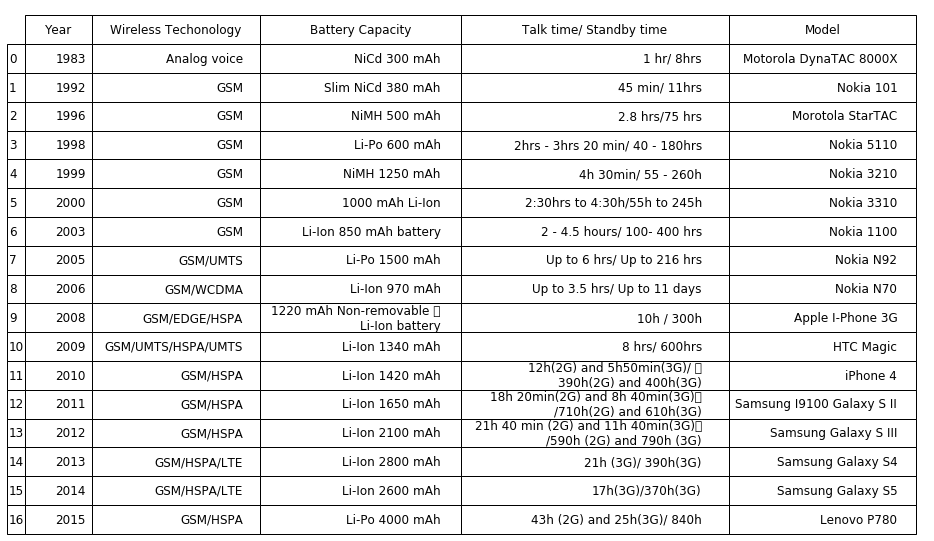
\includegraphics[width=1.4\textwidth, height = 450pt]{MainTable.png}}%
  \caption{Revolution of Cellphone Batteries}
  \label{2}
\end{figure}

We took the battery type of each cellphone and found its voltage. Using both the Milliamps and Voltage of each individual battery, we calculate the battery's watts per hour using the following equation: \par
$$ W = A \cdot V $$ 

\begin{figure}[!ht]
    \makebox[\textwidth][c]{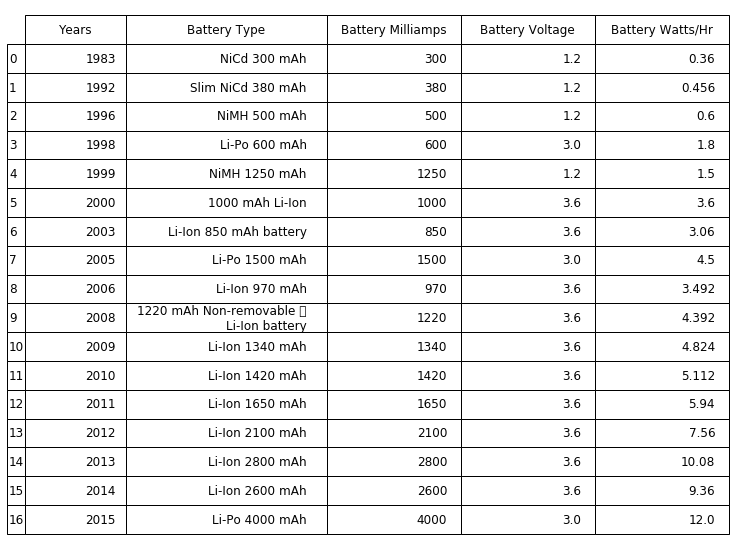
\includegraphics[width=1.4\textwidth, height = 450pt]{Table2.png}}
    \caption{Calculation of Battery Watts per hour}
    \label{3}
\end{figure}

Using our general equation of energy consumption and the data from Figure \ref{2} and Figure \ref{3}, we calculated the energy consumed based on each cell-phone's specific time frame.

\begin{figure}[!ht]
    \makebox[\textwidth][c]{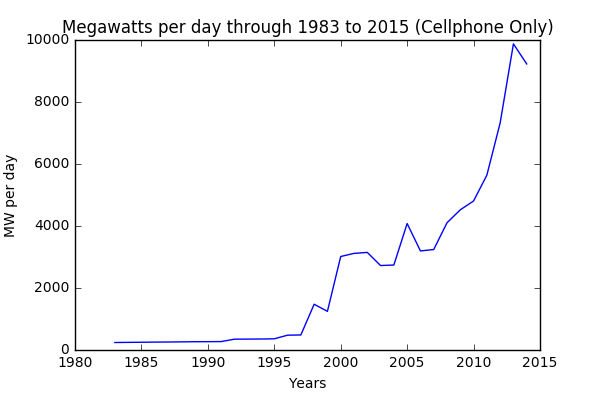
\includegraphics[width=\textwidth, height = 200pt]{CellsOnly.png}}
    \caption{Energy Consumed based on Cells Only}
    \label{4}
\end{figure}

From the looks of Figure \ref{4}, if there were no transition state, the amount of energy consumed would have stayed roughly the same from the time the cell phone was invented till the year $1995$, it would have then started to increase slightly until $2000$, stayed the same for almost $3$ years, decreased a little, spiked again in $2005$, dropped and then skyrocketed from $2006$ onwards. In fact, if looked at it the right way, this graph looks almost like an exponential growth graph. It starts off increasing at a very small rate and then beyond a certain threshold, skyrockets.\par 
Unlike Figure 1 which is increasing linearly, Figure 4 has some dips across the graph. Since the population of the US is always increasing and the number of cellphones is proportional to the population, there shouldn't be any decrease in energy consumption! However, looking at Figure 3, we can see that overall, the wattage of each cellphone throughout the year is increasing. However, upon closer inspection, there are some year intervals that the total wattage of cellphones decrease. Ex: 1998 to 1999, 2005 to 2006, 2013 to 2014... If we correspond these intervals with Figure 4, we can locate the exact position of the dips. Therefore we conclude that these dips are made possible due  to the increased efficiency of technology in these particular year intervals.\par
Another very interesting fact about this graph and the one that came before is that for all the years prior to $2011$, $2012$ the amount of energy consumed if only landlines were in use, is always greater than the amount of energy used if only cell-phones were in use.

\subsubsection{Assume Popularity Index Variation Over Time}
In the previous two steps, we considered our problem in a United States where there is no mixture of households with cell phones and those with landlines. In this step, we begin to consider the more realistic situation where there is a transition period through which members of households begin to replace their landline with cellphones.\par 
We need to point out a few reminders we made at the beginning of this section however. Remember that each household holds $3$ members and that in the starting state, the household utilizes one landline. Moreover, remember that even though we have different versions of cell phones over time in our model, we assume that one model that seemed to dominate the others over a certain period of time is the one we are going to use in our energy consumption calculations.\par 

Let the \textit{popularity-index} of cell phones be a fixed number $p$ in each time step, assuming everyone starts off with a landline, we will choose a random number $n$ associated with each household, and if this $n < p$, then a member of the household in question will go ahead and buy a cell phone. When all members of a household owns a cellphone, they will remove their landline. So then we will calculate the energy associated with landlines, cell phones and both of them combined in this period of time by following this formula: 

$$ E_t = E_u \cdot t \cdot H $$

where $E_t$ is the total energy consumed per day, $E_u$ is the amount of energy consumed by one unit (cell phone or landline) and $t$ is the amount of time the unit is left charging. In our case, we are assuming that each person charged just enough to fill the battery therefore we let $t = 2$. \par 
The visualization of the model of energy consumption explained above leads to the following graph:

\begin{figure}[!ht]
    \makebox[\textwidth][c]{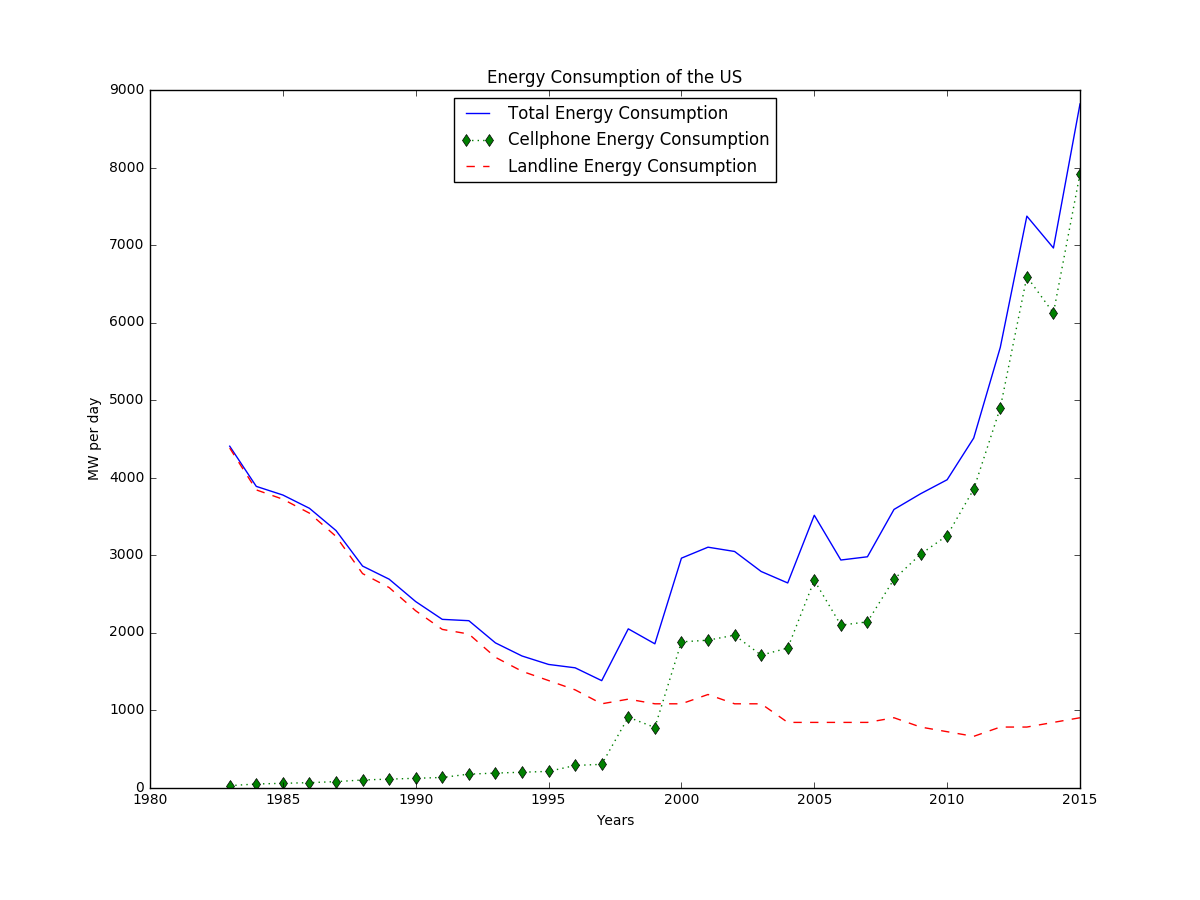
\includegraphics[width=\textwidth + 100pt, height = 250pt]{ElectricConsump01.png}}
    \caption{Energy Consumption with $p = 0.1$}
    \label{5}
\end{figure}

From the graph above, we see landline energy consumption decreasing but it does not reach zero. In fact, we can see it reaching equilibrium at around 3000 MW per day. The cause for this equilibrium could be how we set up our model. To simulate the population growth, we are inputting households into our model. However, these households always start out with one landline and zero cellphones. Therefore this input of one landline will eventually balance out with the rate of transition of landline to cellphones when $p = 0.1$. \par
One might wonder how the graph would change if we increase $p$. Of course, if one understands the concept of the value, he/she can predict how the graph is going to change. In our case, we hypothesize that by increasing the popularity-index of cell phones, the cell phones would grow much quicker while the landlines would go to zero much quicker as well. Decreasing the index would have the opposite effect. For example, the graph below visualizes the change when the popularity index is $0.5$.\par

\begin{figure}[!ht]
    \makebox[\textwidth][c]{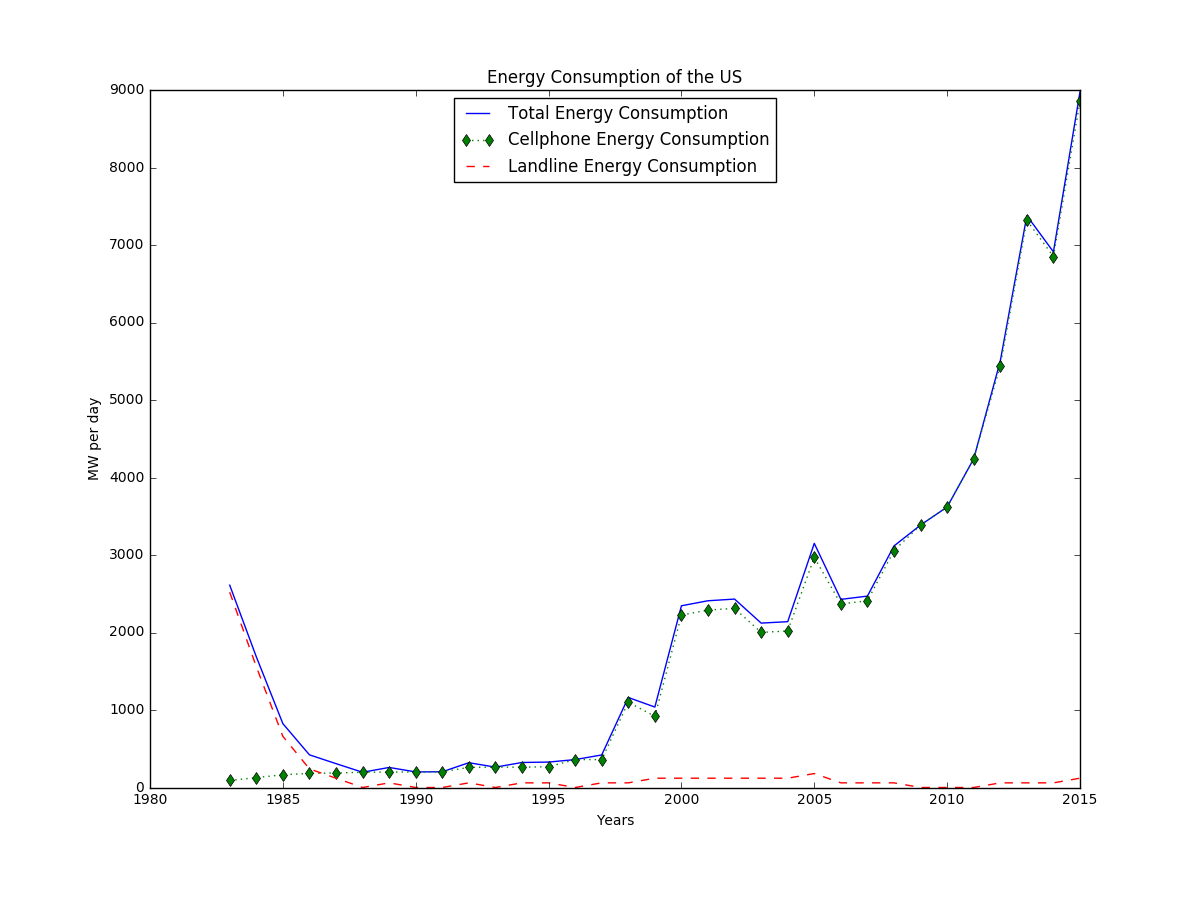
\includegraphics[width=\textwidth + 100pt, height = 250pt]{ElectricConsump05.png}}
    \caption{Energy Consumption with $p = 0.5$}
    \label{6}
\end{figure}

Comparing this graph with Figure \ref{5}, the Total Energy Consumption graph sticks closer to the Cellphone Energy Consumption graph, while the Landline Energy Consumption decreases rapidly.This is to be expected since as the population index increase, people have an increased tendency to replace their landlines with cellphones.\par

The previous two steps hold the \textit{popularity-index} as a constant. We decided to allow the \textit{popularity-index} to change dynamically based on trends of the cellphone. We simulate the popularity index by extrapolating the tread from cellphone subscribers in the US. \cite{subscribers} \par

\begin{figure}[!ht]
    \makebox[\textwidth][c]{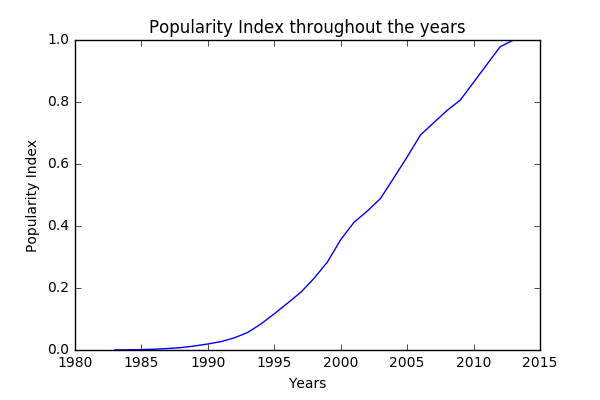
\includegraphics[width=\textwidth]{PopularityIndex.png}}
    \caption{Trend of Popularity Index}
    \label{7}
\end{figure}

The graph above shows a logistic curve as the growth slowly increases in the first 15 years. After 1995, the popularity of cellphones suddenly increases rapidly until 2014 where is slowly levels out. \par

If we integrate this dynamic popularity index into our graph, what we get is Figure \ref{8}.\pagebreak

\begin{figure}[!ht]
    \makebox[\textwidth][c]{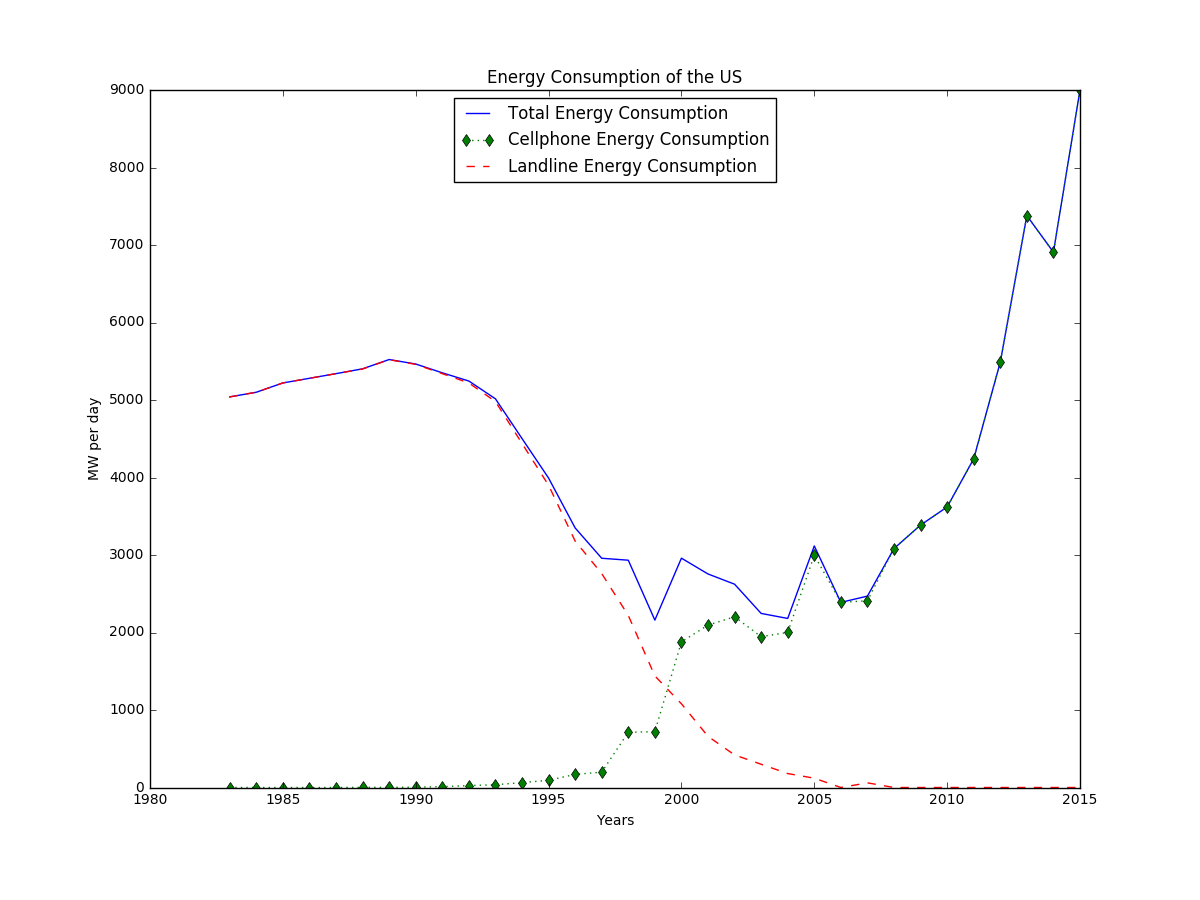
\includegraphics[width=\textwidth]{ElectricConumpPop.png}}
    \caption{Dynamic Popularity Index on Electric Consumption}
    \label{8}
\end{figure}

The landline energy consumption shows a logistic declination while the cellphone energy consumption still rises exponentially. However, the important part of Figure \ref{8} is the Total energy consumption. In fact, throughout the years, total energy consumption is not purely increasing. When landline's popularity was at its peak, energy consumption was actually moderately high. It was until year 2004 to 2005, there is a optimal mix between landlines and cellphones in the US where the global minimum of total energy consumption occur. After 2005, total energy consumption increases rapidly and has no signs of slowing.

To close this section off, among our results, we have the fact that energy consumption due to phone-service usage, if the cell phone had not been invented would have been growing linearly. We also know that this figure has been growing exponentially (not taking into account the dips in the graph due to the change of phone model) over time. Moreover, as one would expect, the number of landline-owning households tend to go to zero over time. \par

\subsubsection{Overcharging}
We assume that if a phone is overcharged, it would use the same amount of energy that it would when charging. So instead of using $2$ hours for our model, we would instead use $8$ hours; the average amount of time for someone to charge overnight. However due to a study \cite{overCharge}, the average wattage used while charging a charged battery is 2.24W. As seen in Figure \ref{overcharging}, there is quite a significant difference if everyone decides to charge their phones overnight.\par

As seen in Figure \cite{overCharge}, overcharging has a significant impact. In 2015, the difference between overcharging and $2$ hours charging is around a 100\%. Even though individually, each household wouldn't spent much energy, in the whole scale of population growth, the meager amount becomes a huge impact.

\begin{figure}
    \centering
    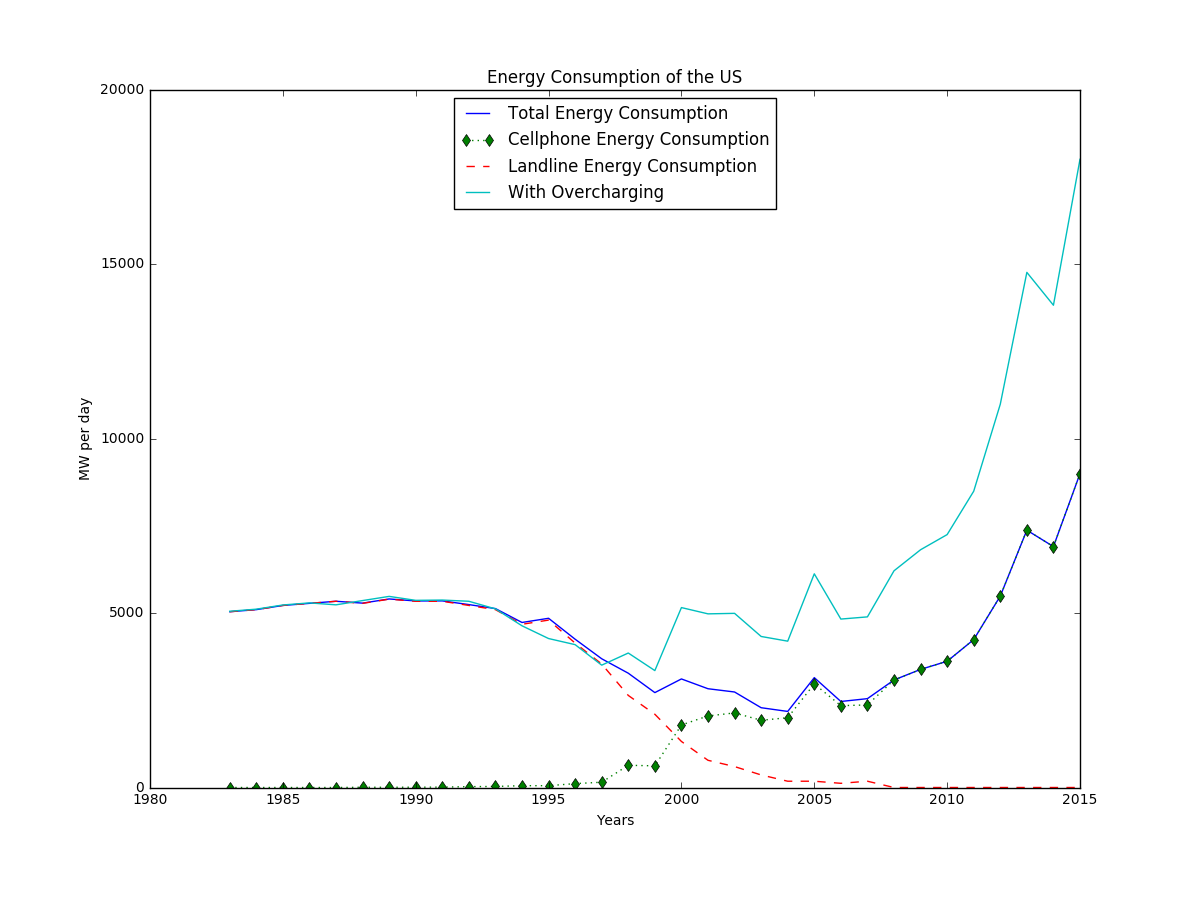
\includegraphics[width=\textwidth]{Overcharging.png} 
    \caption{Total Energy Consumption with Overcharging}
    \label{overcharging}
\end{figure}


\subsection{Differential Equations Modeling}
As we have briefly described already, differential equations modeling takes a somewhat different approach when solving problems than Monte Carlo simulations do. Whereas Monte Carlo simulations, in one way or another, use randomness to describe an overall change of a system, differential equations modeling first looks at the whole systems, and their interactions between each other, comes up with differential equations describing the interactions among the systems and then does the plotting and analysis of results.\par 
In order to do this, what is often done is to use \textit{compartment models} as a way to visualize the system of populations one wants to deal with. In this case, our populations can be thought of as the amount of landlines as well as the amount of cell phones in the United States at a given point in time.\par 

For this model we are developing, our compartment model is quite simple since we only have land-line owning households turning into cell phone owning households.
It can be visualized as in Figure \ref{9}.

\begin{figure}
    \centering
    
\includegraphics[width=\textwidth]{compartment.png} 
    \caption{Compartment Model}
    \label{9}
\end{figure}

The role of compartment models in differential equations modeling is to provide us with a simple way to visualize our systems as well as an easy way to produce differential equations representing the different changes that happen inside our systems. \par 

Using our compartment model above, we get the following equations as a result.

\begin{align*}
    \frac{dL}{dt}  &= -\upalpha L \\
    \frac{dT}{dt}  &= \upalpha L - \upvarsigma T \\
    \frac{dC}{dt}  &= \upvarsigma T + \beta H\\
    \frac{dH}{dt}  &= 1.3 
\end{align*}



Where $L$ is the total number of households with landlines and no cell phones in the US, $T$ is the total number of households with landlines and cell phones, $C$ is the total number of households with only cell phones and no landlines, and $H$ is the total number of households in the United States. $\upalpha, \upvarsigma, $ and $\beta$ are landline-decrease parameter, popularity-index and new-phone-service users parameter respectively. This is a good place to note that, in our model we assume that no one buys a landline after the invention of the cell phone. So, the increase in population only affects the number cell-phone possessing households as reflected in the differential equations. The rate of change of the population per year has been obtained as described next.\par 

\begin{figure}
    \centering
    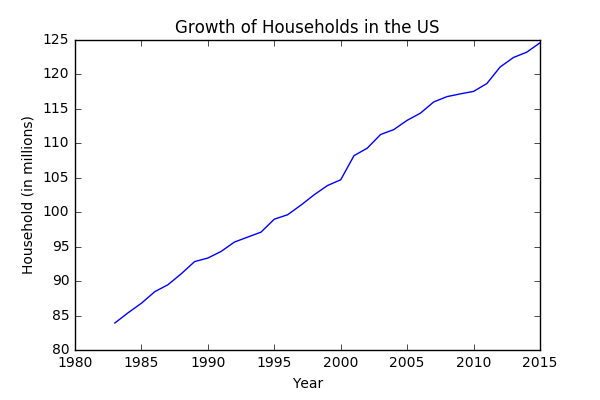
\includegraphics[width=\textwidth]{HouseholdGrowth.png} 
    \caption{Growth of Households}
    \label{10}
\end{figure}
 
 The plot obtained through considering data from Statistica \cite{Households} about population growth in the United States, looks like shown in figure \ref{10}. Clearly, this graph describes a linear growth. And in fact, taking the first and the last point, that is $(1985, 85)~ \text{and} ~(2015, 125)$, from this graph gives us a $1.3$ slope which we then take as the slope of the whole graph and use it as the rate of change of the the population in our differential equations. \par 

Moreover, note how in the differential equations above only the number of cell phones at any given point in time actually depends on the number of households. This is because the number of households with only landlines, and the number of households with both cell phones and landlines only depend on the initial amount of households and not the actual amount of households at a specific time.\par

Initially, as provided by Statistica \cite{Households}, there are $83$ million landline-owning households in the United States. At the same point in time, there are zero housed transitioning from landlines to cell phones, and there are zero cell-phone owning households. However, the next year, all the values start to change following our model in which the parameters, $\upalpha, \upvarsigma, $ and $\beta$ are set to $0.3$, $0.1$, as in the other model, and $0.05$ respectively. That is to say that $30\%$ the landline owning population convert to cell phones every year, $10\%$ of households that were in transition become fully cell phone owning, and that only $1\%$ of the new population buy cell phones. By taking these parameters and starting conditions into account,  the resulting overall graph is shown in figure \ref{11}.\par 

\begin{figure}
    % \centering
    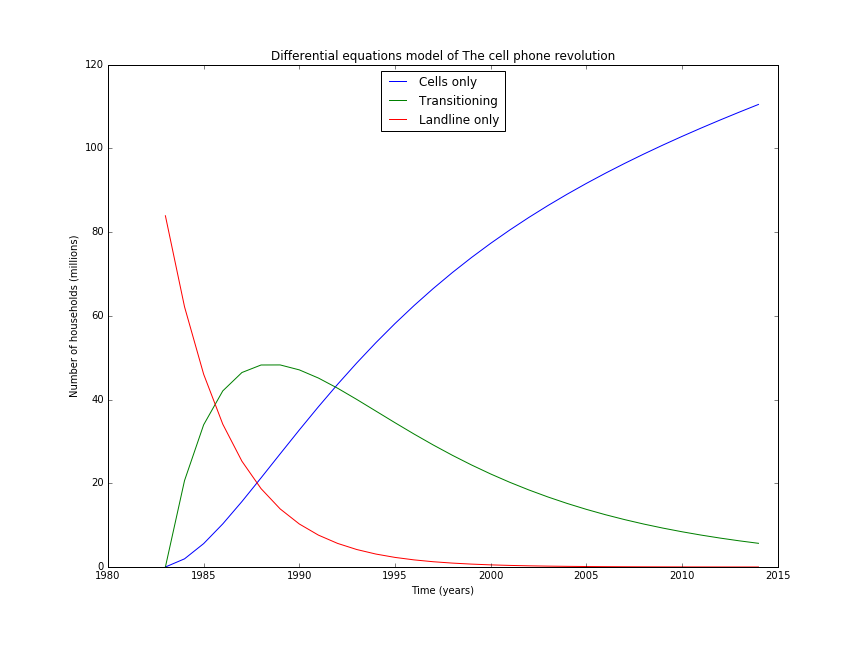
\includegraphics[width=\textwidth]{Differential1.png} 
    \caption{Phone Service Over Time}
    \label{11}
\end{figure}

As one would expect, from the graph, we see that the overall change in our system can be described as follows. Since the day cell phones were invented, their numbers have been increasing according to a logistic growth described by the graph. The number of households in the transition state start by increasing from zero until they reach their maximum in $1990$ and then start going down like the landlines.\par 
Using the amount of energy consumed per household found in the previous section over the years as well as the energy consumption of each popular cell phone like we did in the previous model but using the results we found from our differential equations modeling for the number of cell phones and the number of landlines over the years, the graph look like it is shown in figure \ref{12}

\begin{figure}
    \centering
    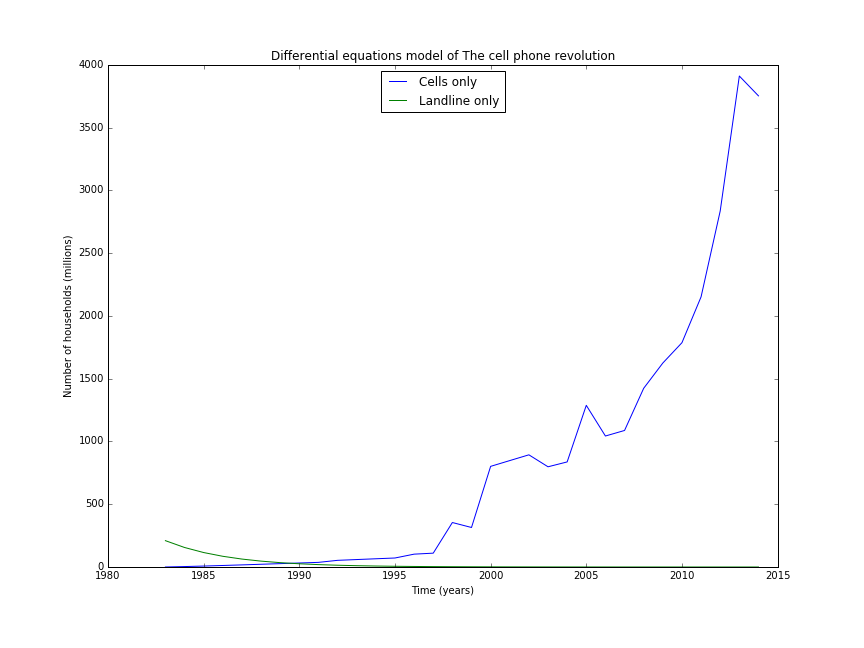
\includegraphics[width=\textwidth]{Differential3.png} 
    \caption{Phone Service Energy Consumption over Time}
    \label{12}
\end{figure}


\section{Sensitivity Testing}
\subsection{Monte Carlo Simulation}
\subsubsection{Popularity-Index}
In our model, we shaped the popularity index so that it varies from 0 to 1. We did not take into consideration values above 1 or any negative values. However, based on the definition of popularity index, a value greater than 1 or less than 0 will not necessarily make our model invalid. If the value is greater than 1, then it means that every member of each household will immediately replace their landline with cellphones. If the value is less than 0, then it means that there is absolutely no tendency for people to get a cellphone. Therefore our model will still be relevant but the results will not be significant.\par
\subsubsection{Popular Phones}
Our model assumes that everyone uses the same phone in a given time period. As mentioned before, we believe this assumption should not affect the results we calculate significantly due to the fact that technology is competitive. If we choose the most popular cellphone in that era, the specs of the other cellphones in that era should not deviate too far away. However if this assumption does not hold true in reality, then our model will not be valid. If our assumption is an overestimation on battery capacity, then in reality, the total consumption of energy might still be increasing but at a slower rate or it might even decline after a certain year. If our assumption is an underestimation, then the US is wasting more energy than expected.\par

\begin{figure}[!ht]
    \centering
    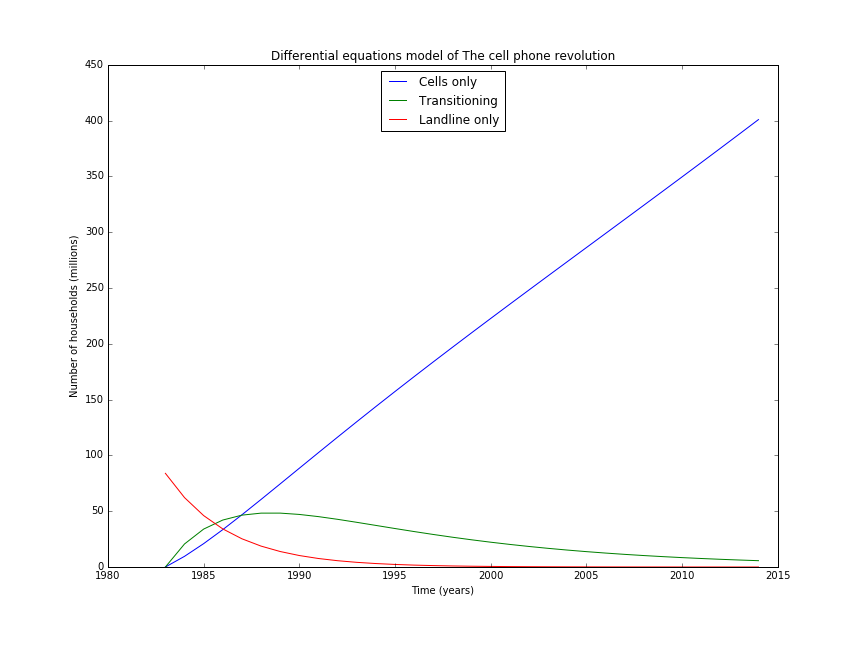
\includegraphics[width=\textwidth]{Differential2.png} 
    \caption{Phone Service Over Time 2}
    \label{13}
\end{figure}

\subsection{Differential Equations}
Our differential equations model is very sensitive. That is to mean that one can get very different results by not changing much to the parameters we use in our differential equations. For example by changing the fraction of new people who buy cell phones from $1\%$ to $10\%$, the increase in cell phone numbers become almost linear.(see figure \ref{13}). Thus, our model tries to be as realistic as we can possibly be which doesn't give use the best results but still gives good results, but this comes at a price of being very sensitive. \par We should mention then, that most of the numbers we choose for use as our parameters are not random. They were, like the \textit{popularity index}, obtained by looking at data from \cite{subscribers}, and finding trends in the data which allowed us to come up with the numbers.\par 
Therefore, even though our model looks only at the United States, the methods we used, and the equations we came up with can be used on any other country, given data about the country and deciding values of the parameters in the equations accordingly.


\section{Evaluation}

From the graphs about energy consumption, that is Figure \ref{12} and Figure \ref{8} as well as Figure \ref{overcharging}, we can see that the graphs agree even though they come from two different models.\par 
The differential model looks at the whole situation which is difficult to get to the specifics. Whereas the Monte Carlo simulation can simulate each household and expand according to scale. However each model has its strength and weaknesses. 

\subsection{Monte Carlo Simulation}
\subsubsection{Strengths}
\begin{itemize}
    \item With accurate data, results tend to be more realistic. What we have modelled agrees with what we have hypothesized.
    \item By using randomness for the transit of landlines to cellphones, we cover the possible errors if we try to model the actual transiting behavior of the US.
\end{itemize}
\subsubsection{Weaknesses}
\begin{itemize}
    \item Unexplainable results may arise based on estimated values. Ex. Dips on Figure 4.
    \item Must model many households in congruence in order to get a reasonable result. Modeling one household using Monte Carlo Simulation will not give us appropriate results.
    \item Harder to predict future results based on current data. We need to find the curve's regression line in order to predict future trends.
\end{itemize}
\subsection{Differential Equations Model}
\subsubsection{Strength}
\begin{itemize}
    \item Easy to expand time frame of model to predict future trends.
\end{itemize}
\subsubsection{Weaknesses}
\begin{itemize}
    \item When modeling a large scale environment, the model tends to be more generalized and cannot encompass specific details that happen.
\end{itemize} 

\section{Conclusion}
From our models, we conclude that our findings are similar to what we have hypothesized. Energy consumption does increase and the main component is the popularity growth in the US. Even if cellphones suddenly become very efficient and takes 80\% less energy to run, there will still be an increasing trend of energy consumption. However, from Figure \ref{8}, we found that energy consumption does not increase absolutely throughout the years. There is an optimum point where energy consumption is at its lowest. If we are to find this optimum, we may be able to advice on how to minimize energy consumption through the different spreads of landlines and cellphones.



\section{Future Work}
Even though our model is able to tell us a lot about how much energy consumption has increased over the last years due the cell phone revolution, it is still not perfect. Below are some of our thoughts as to how we might improve our model:

\begin{itemize}
    \item 
    Find an optimal way of providing phone service, minimizing energy consumption.
    
    \item 
    Taking into account economic and population growth over the next 50 years or so, give a scientifically backed prediction of the energy needs of providing phone service.
\end{itemize}

\begin{thebibliography}{7}
\bibitem{Households}
Statistica: Number of Households in the United States.\\
\texttt{https://www.statista.com/statistics/183635/number-of-households-in-the-us/}

\bibitem{subscribers}
Info Please: Cell Phone Subscribers in the U.S., 1985–2010.
\texttt{http://www.infoplease.com/ipa/A0933563.html}

\bibitem{phoneBatteries}
Pandikumar, S. and M.Sumathi M.Sumathi. "Investigation On The Revolution And Need Of Energy Efficient Smartphone Development". International Journal of Computer Applications 117.11 (2015): 1-5. Web.
\texttt{http://research.ijcaonline.org/volume117/number11/pxc3903091.pdf}

\bibitem{AverageSizeHousehold}
"Average Size Of Households In The U.S. 1960-2015 | Statistic". Statista. N.p., 2016. Web. 15 Nov. 2016.
\texttt{https://www.statista.com/statistics/183648/average-size-of-households-in-the-us/}

\bibitem{chargerData}
Trollinger, Vernon. "How Much Energy Does My Phone Charger Use?". Bounce Energy Blog. N.p., 2016. Web. 16 Nov. 2016.
\texttt{http://www.bounceenergy.com/blog/2016/02/how-much-energy-does-this}
\texttt{-appliance-use-phone-charger/}

\bibitem{overCharge}
"Standby Power : Data". Standby.lbl.gov. N.p., 2016. Web. 9 Dec. 2016.
\texttt{http://standby.lbl.gov/summary-table.html}

% \bibitem{}

\end{thebibliography}






\end{document}
